\chapter{Pengujian Sistem RaspberryPi}

\begin{figure}[ht]
  \centering
  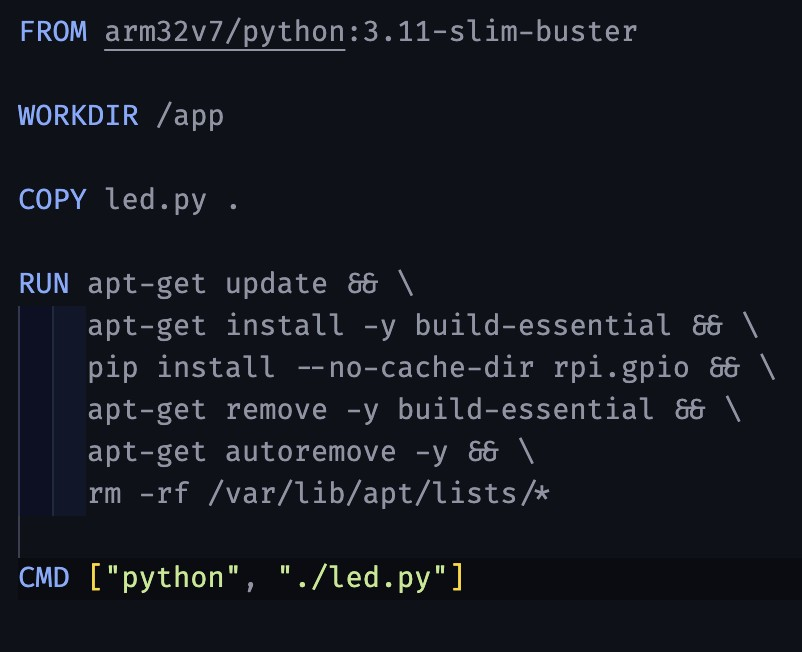
\includegraphics[width=0.8\textwidth]{resources/chapter-4/pengujian/pengujian-sistem-raspi-09-dockerfile.jpg}
  \caption{Python Docker LED Script}
  \label{fig:raspi-docker-led-script}
\end{figure}

\begin{figure}[ht]
  \centering
  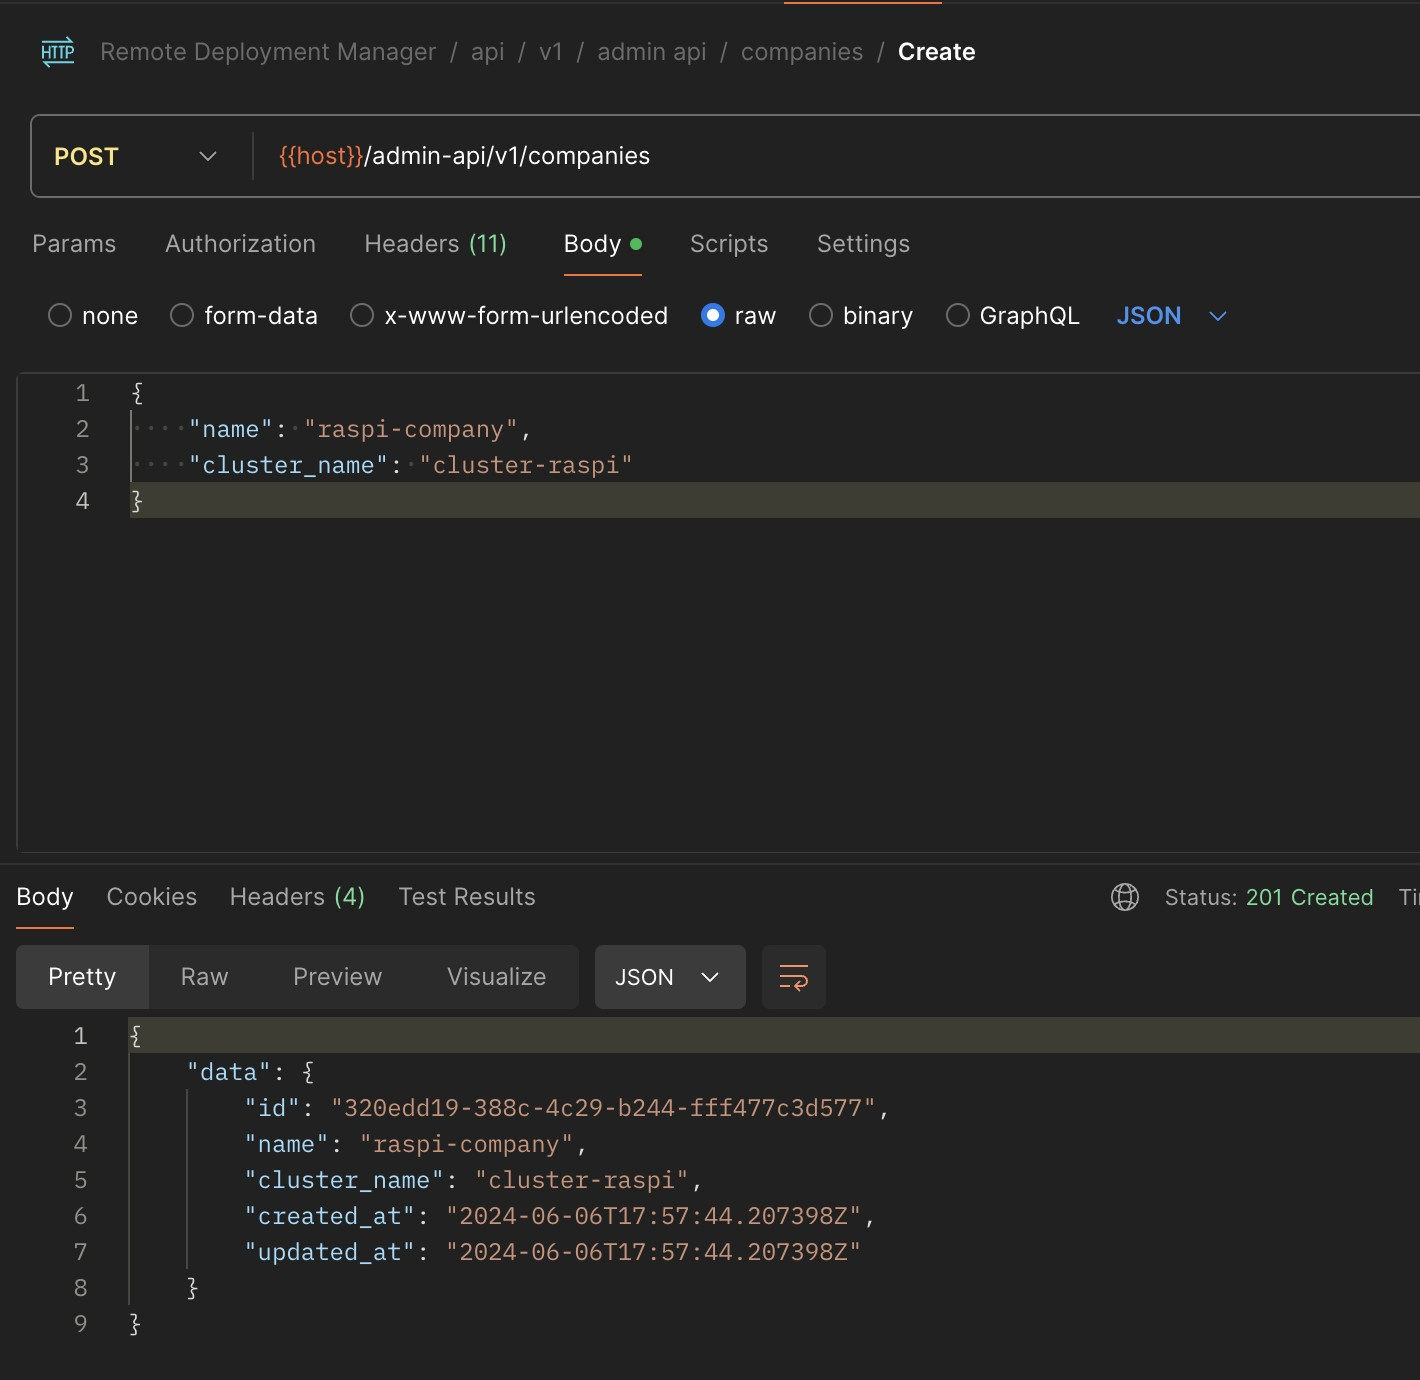
\includegraphics[width=0.8\textwidth]{resources/chapter-4/pengujian/pengujian-sistem-raspi-01.jpg}
  \caption{Pembuatan \textit{Company} Raspi Company}
  \label{fig:pengujian-sistem-raspi-01}
\end{figure}

\begin{figure}[ht]
  \centering
  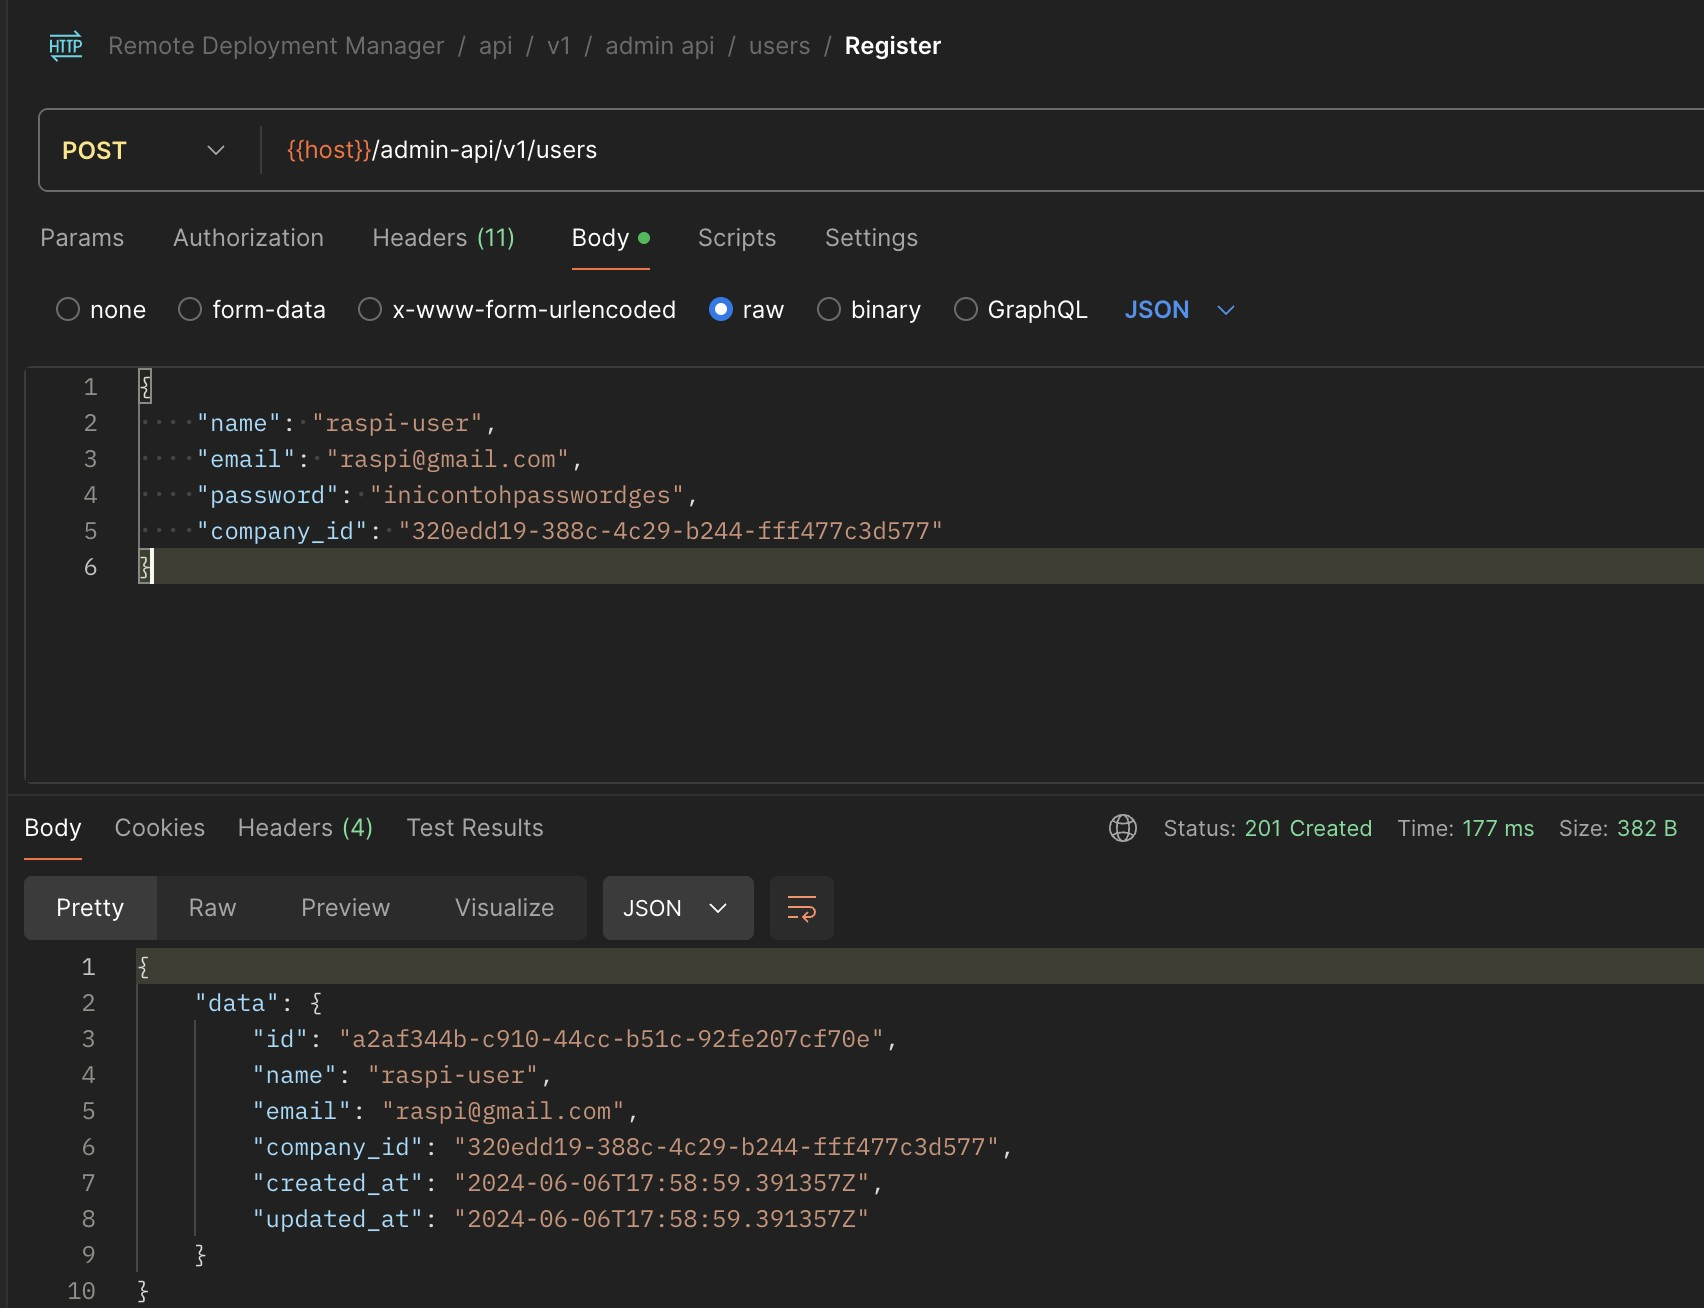
\includegraphics[width=0.8\textwidth]{resources/chapter-4/pengujian/pengujian-sistem-raspi-02.jpg}
  \caption{Pembuatan \textit{User} Raspi-User}
  \label{fig:pengujian-sistem-raspi-02}
\end{figure}

\begin{figure}[ht]
  \centering
  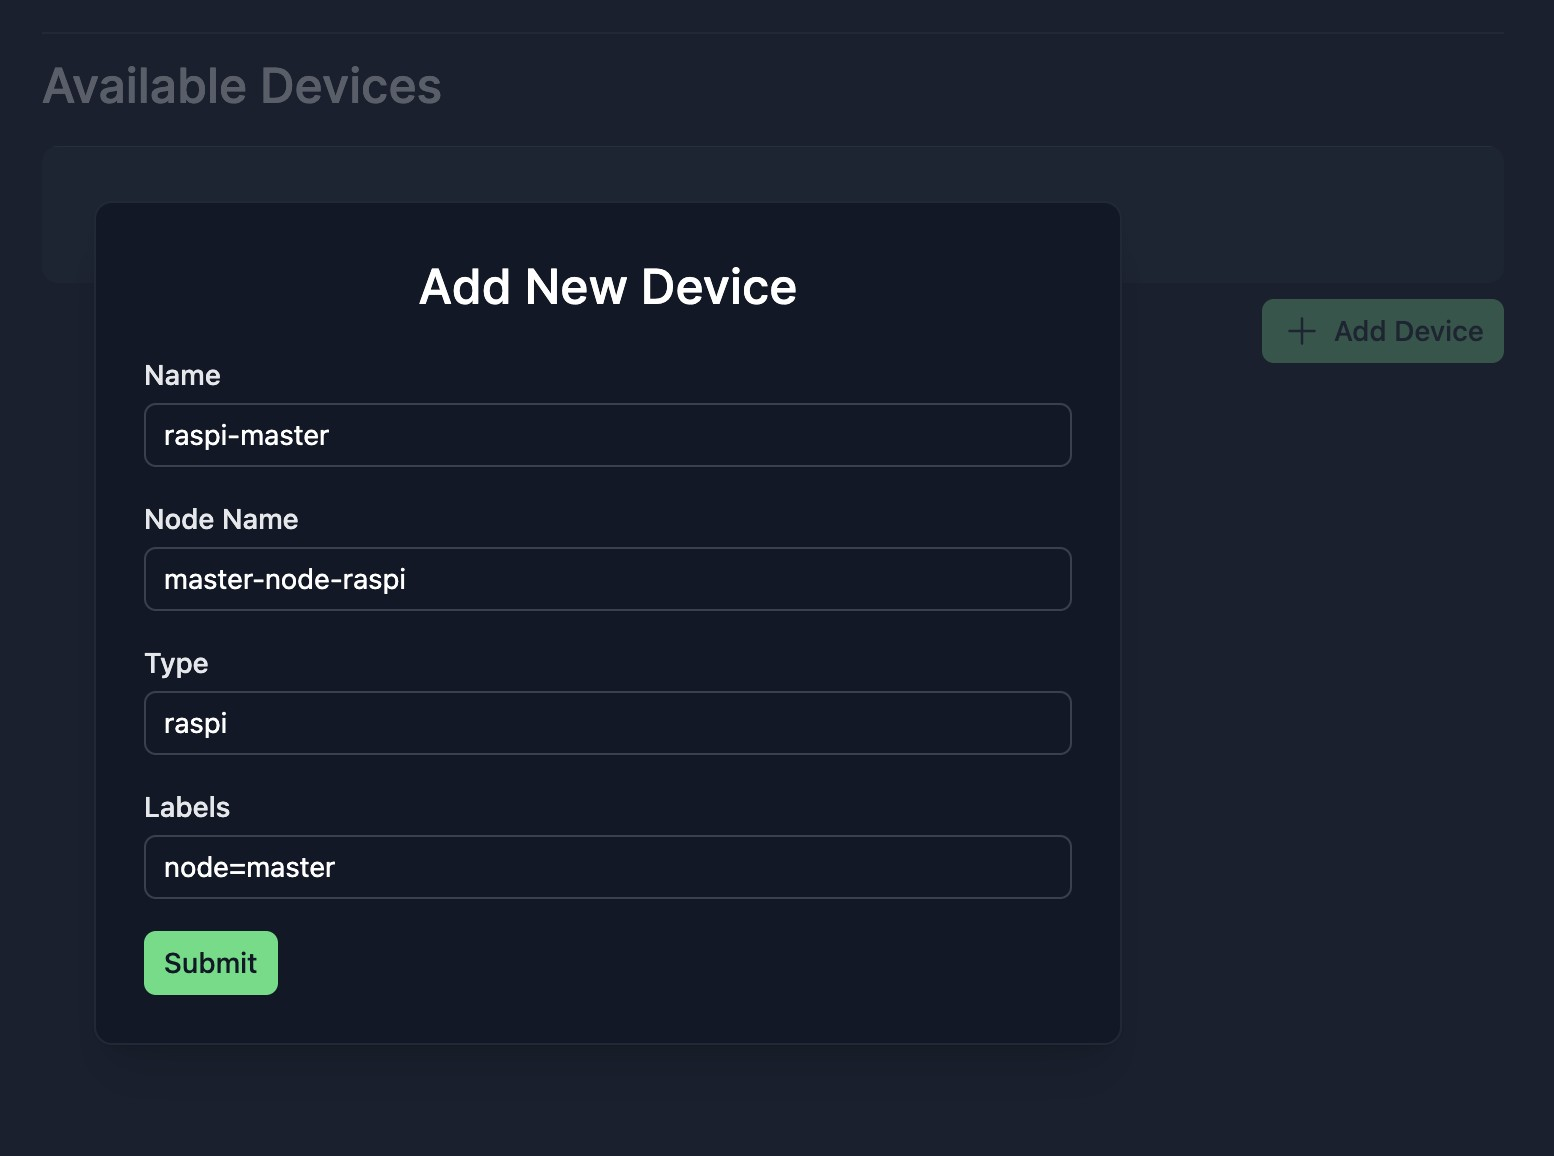
\includegraphics[width=0.8\textwidth]{resources/chapter-4/pengujian/pengujian-sistem-raspi-04-1.jpg}
  \caption{Pembuatan \textit{Device} Raspi}
  \label{fig:pengujian-sistem-raspi-04}
\end{figure}

\begin{figure}[ht]
  \centering
  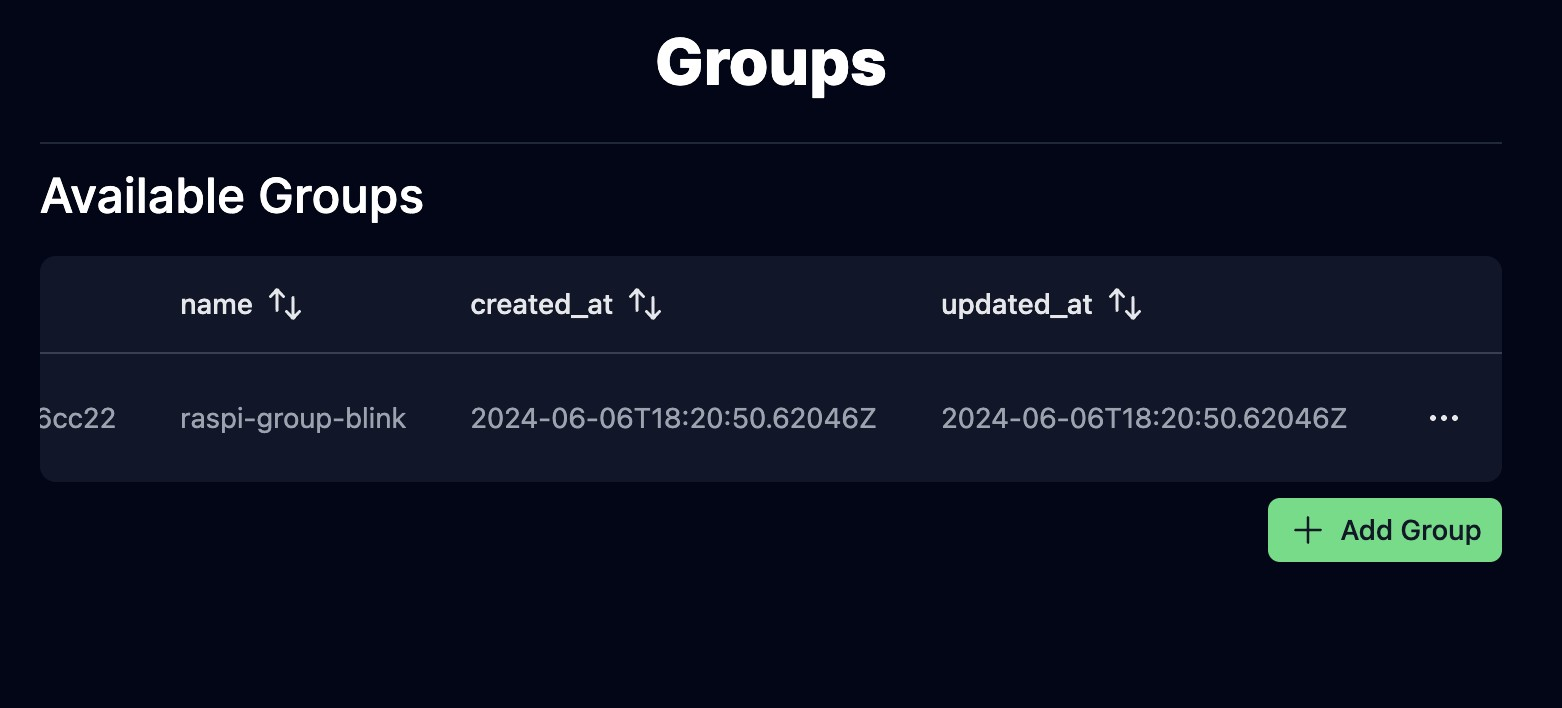
\includegraphics[width=0.8\textwidth]{resources/chapter-4/pengujian/pengujian-sistem-raspi-05.jpg}
  \caption{Pembuatan \textit{Groups} Raspi}
  \label{fig:pengujian-sistem-raspi-05}
\end{figure}

\begin{figure}[ht]
  \centering
  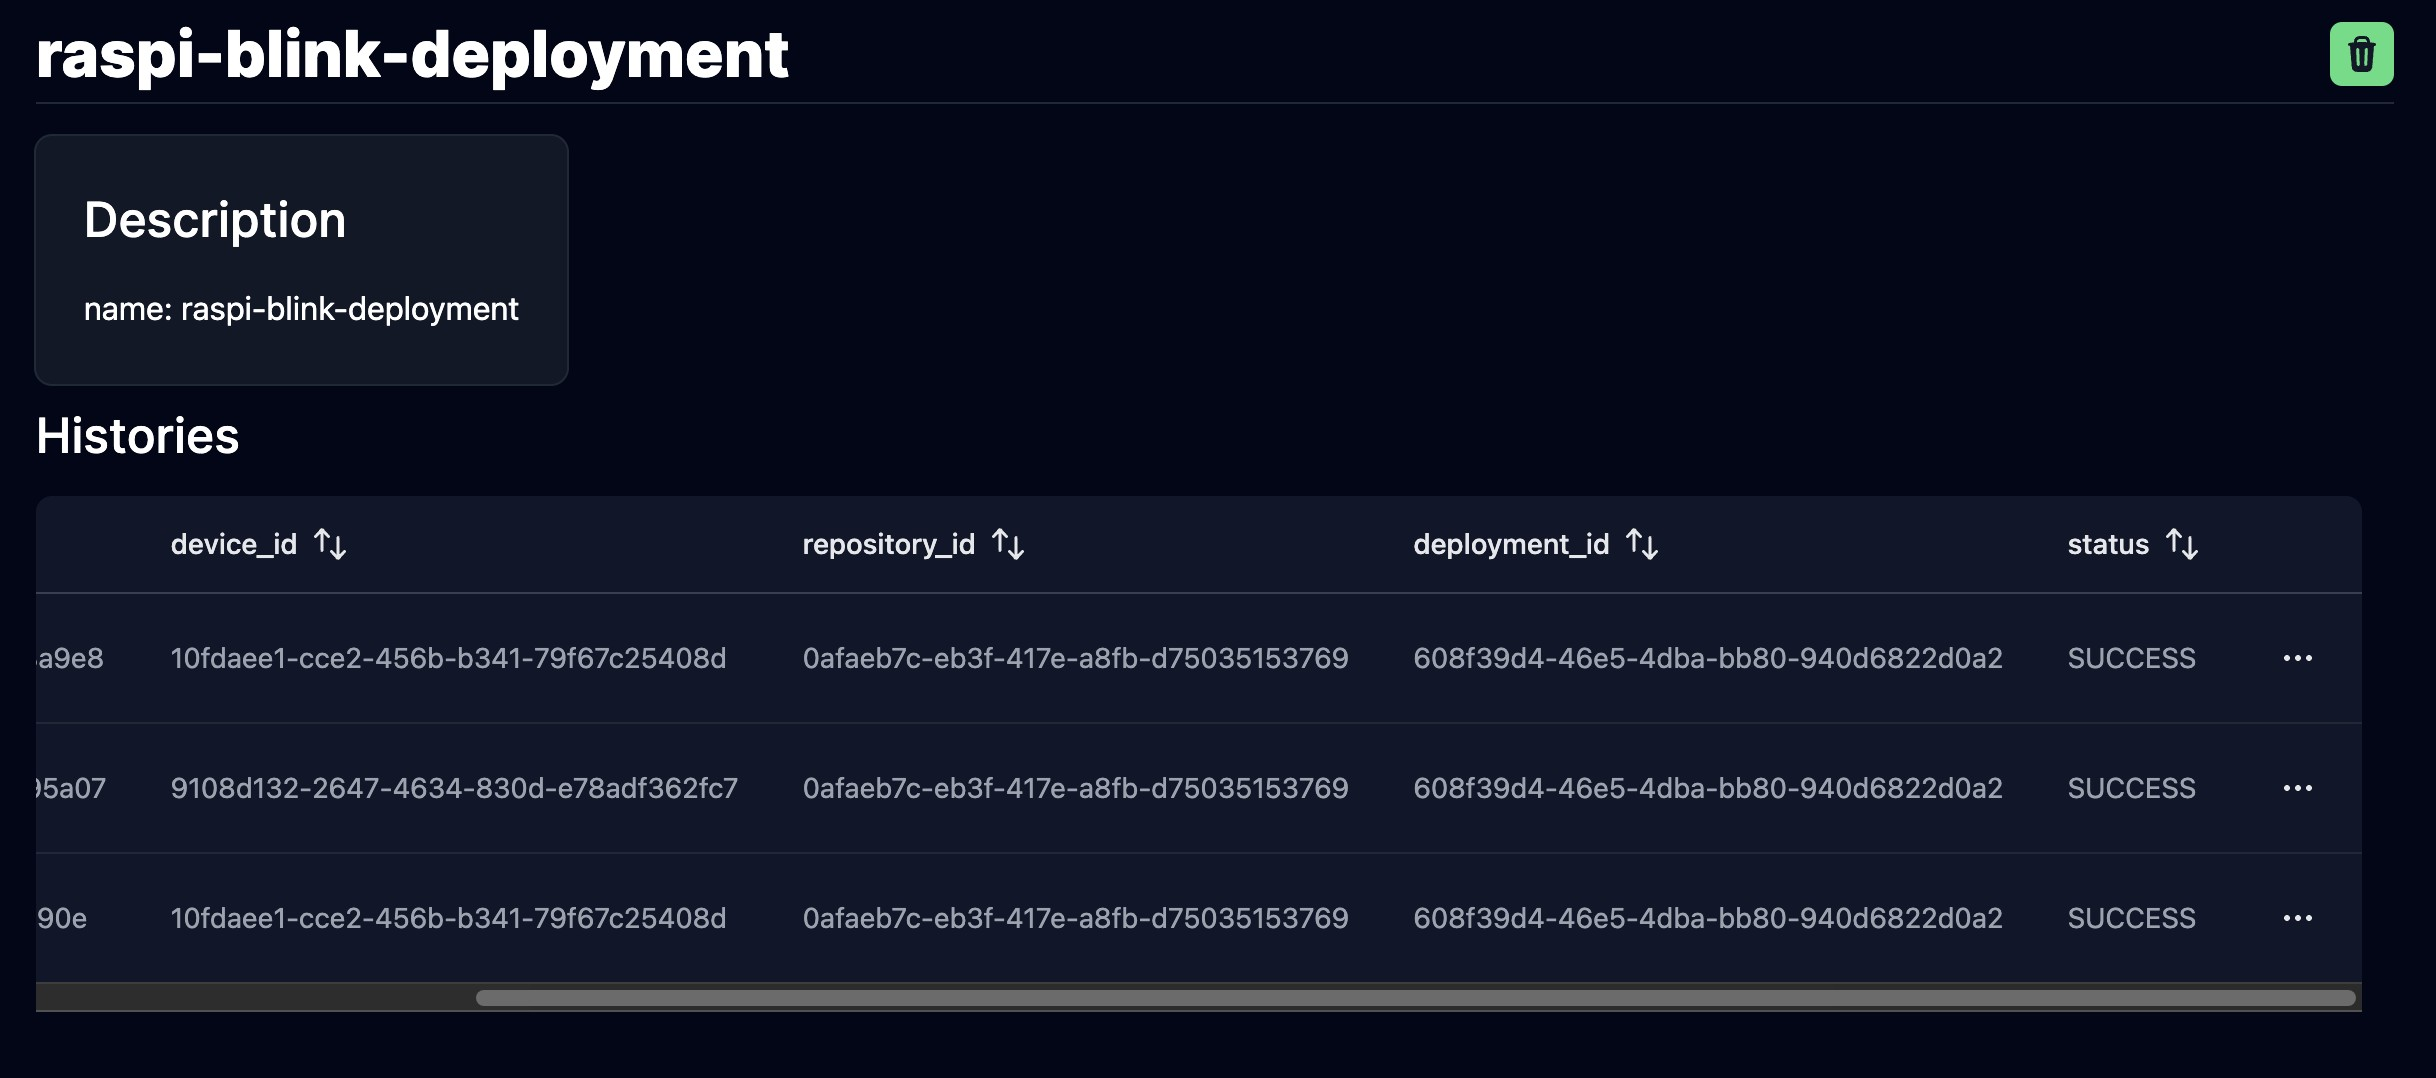
\includegraphics[width=0.8\textwidth]{resources/chapter-4/pengujian/pengujian-sistem-raspi-10.jpg}
  \caption{Riwayat \textit{deployment} "raspi-deployment-bink"}
  \label{fig:pengujian-sistem-raspi-10}
\end{figure}

\begin{figure}[ht]
  \centering
  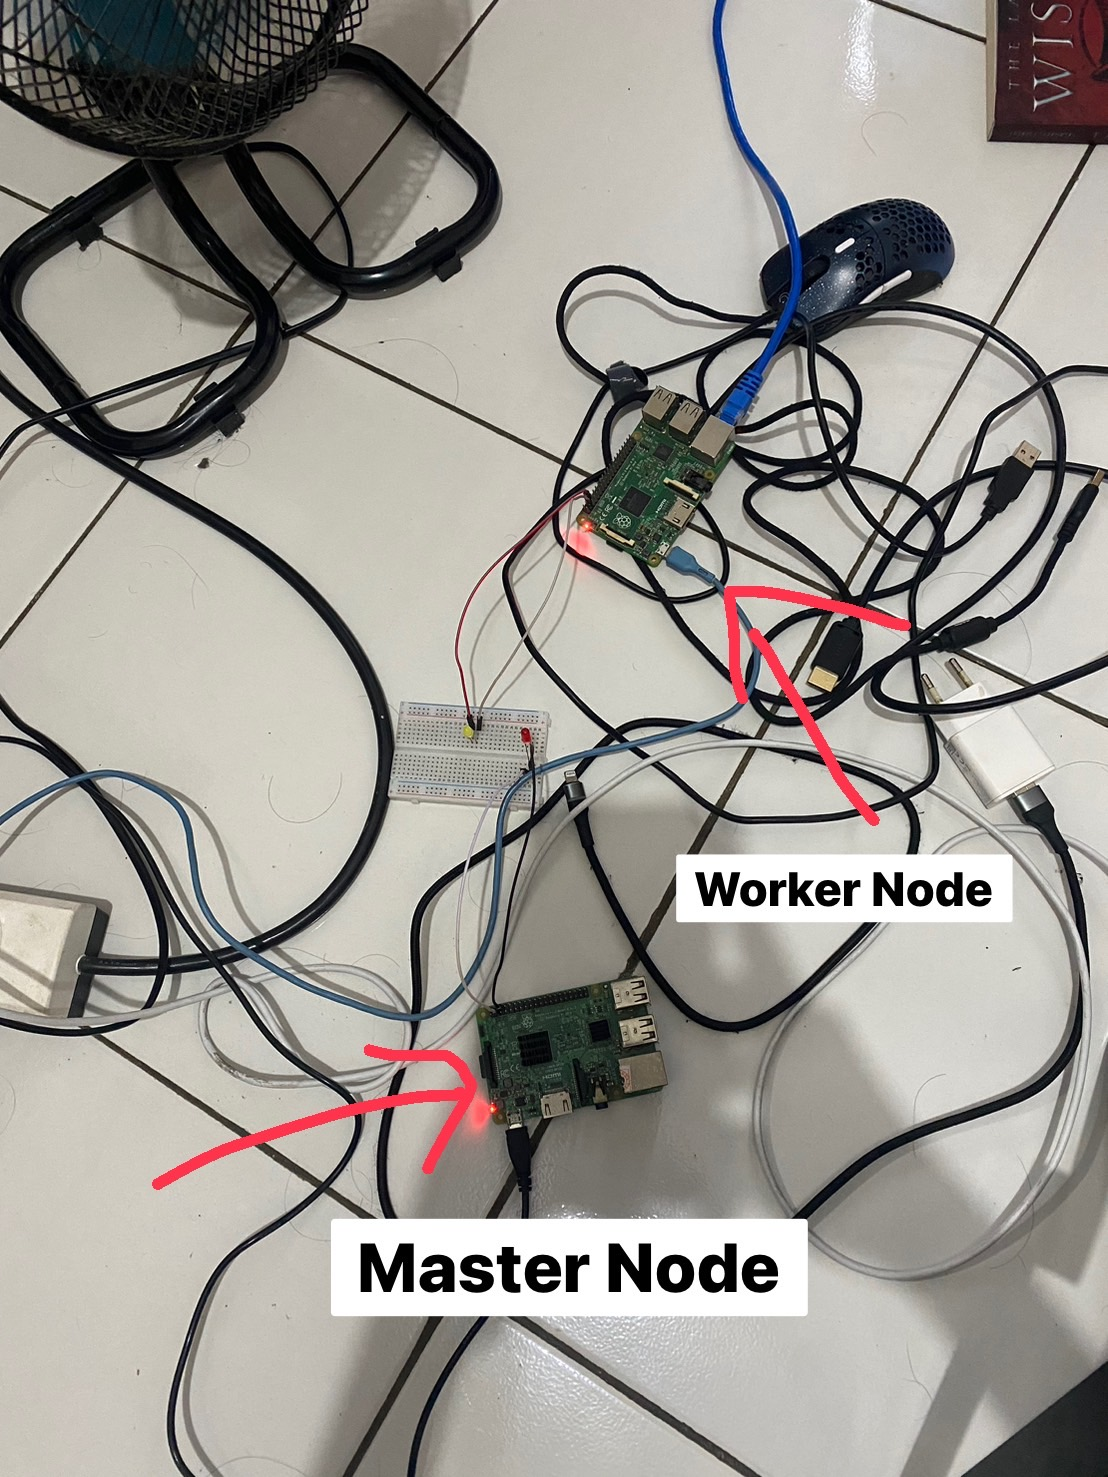
\includegraphics[width=0.8\textwidth]{resources/chapter-4/pengujian/pengujian-sistem-raspi-layout.jpg}
  \caption{Layout Sederhana \textit{Clustser} RaspberryPi}
  \label{fig:pengujian-sistem-raspi-layout}
\end{figure}

\begin{figure}[ht]
  \centering
  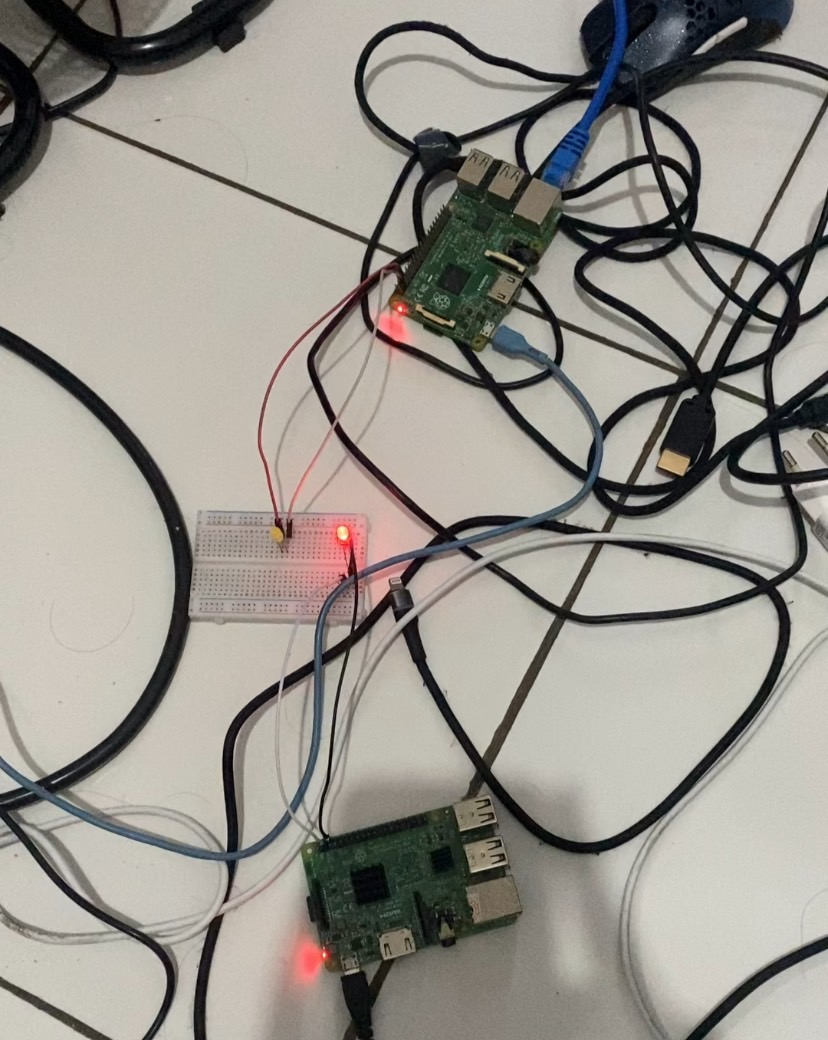
\includegraphics[width=0.8\textwidth]{resources/chapter-4/pengujian/pengujian-sistem-raspi-hasil-a.jpg}
  \caption{Hasil Pengujian Sistem Target Deployment Raspi}
  \label{fig:hasil-pengujian-sistem-raspi-target}
\end{figure}

\begin{figure}[ht]
  \centering
  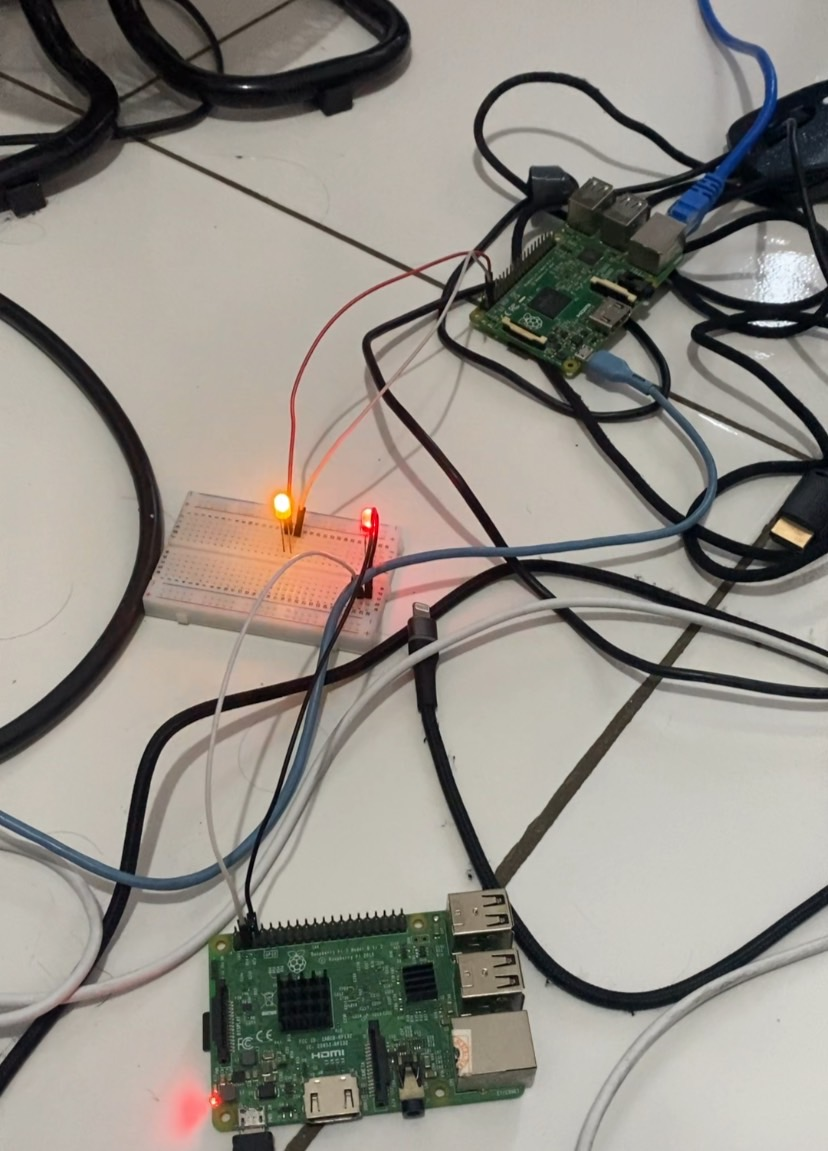
\includegraphics[width=0.8\textwidth]{resources/chapter-4/pengujian/pengujian-sistem-raspi-hasil-b.jpg}
  \caption{Hasil Pengujian Sistem Custom Deployment Raspi}
  \label{fig:hasil-pengujian-sistem-raspi-custom}
\end{figure}

\bgroup
\begin{table}[ht]
  \def\arraystretch{1.3}
  \caption{Skenario dan Hasil Pengujian Sistem \textit{RaspberryPi}}
  \label{tab:pengujian-sistem-raspi}
  \centering
  \begin{tabular}{|p{2cm}|p{2cm}|p{4cm}|p{3cm}|p{2cm}|}
    \hline
    \centering{ID Fungsional} & \centering{ID Pengujian}                            & \centering{Skenario}                                                                           & \centering{Ekspektasi}                                                                    & Realita \\
    \hline
    F01                       & P20                                                 & \textit{Admin} membuat \textit{company} yang dengan nama "raspi-company"                       & \textit{Admin} berhasil mendaftarkan \textit{company}                                     & Sesuai  \\
    \hline
    F04                       & P21                                                 & \textit{Admin} membuat \textit{user} yang dengan email "raspi@gmail.com"                       & \textit{Admin} berhasil mendaftarkan \textit{user}                                        & Sesuai  \\
    \hline
    F06                       & P22                                                 & \textit{User} ingin login dengan kredensial "raspi@gmail.com"                                  & \textit{User} berhasil login ke dalam sistem                                              & Sesuai  \\
    \hline
    F10                       & P23                                                 & \textit{User} mendaftarkan dua \textit{devices} dengan nama "raspi-master" dan
    raspi-worker"             & \textit{User} berhasil mendaftarkan \textit{device} & Sesuai                                                                                                                                                                                               \\
    \hline
    F13                       & P24                                                 & \textit{User} mendaftarkan \textit{group} dengan nama "raspi-group-blink"                      & \textit{User} berhasil mendaftarkan \textit{group}                                        & Sesuai  \\
    \hline
    F16                       & P25                                                 & \textit{User} mendaftarkan \textit{device} pada \textit{group} dengan nama "raspi-group-blink" & \textit{User} berhasil mendaftarkan \textit{device} ke \textit{group} "raspi-group-blink" & Sesuai  \\
    \hline
    F17                       & P26                                                 & \textit{User} mendaftarkan \textit{deployment images} dengan nama "raspi-image-blink"          & \textit{User} berhasil mendaftarkan \textit{deployment images}                            & Sesuai  \\
    \hline
  \end{tabular}
\end{table}
\egroup

\bgroup
\begin{table}[ht]
  \def\arraystretch{1.3}
  \centering
  \begin{tabular}{|p{2cm}|p{2cm}|p{4cm}|p{3cm}|p{2cm}|}
    \hline
    \centering{ID Fungsional} & \centering{ID Pengujian} & \centering{Skenario}                                                                                                                                                                                                                  & \centering{Ekspektasi}                                                 & Realita \\
    \hline

    F18                       & P27                      & \textit{User} melihat daftar \textit{deployment images} yang tersedia dengan mengunjungi halaman /deployments                                                                                                                         & \textit{User} berhasil melihat daftar \textit{deployment images}       & Sesuai  \\
    \hline
    F20                       & P28                      & \textit{User} membuat \textit{deployment plan} dengan nama "raspi-deployment-blink"                                                                                                                                                   & \textit{User} berhasil membuat \textit{deployment plan}                & Sesuai  \\
    \hline
    F21                       & P29                      & \textit{User} melihat daftar \textit{deployment plan} yang tersedia dengan mengunjungi halaman /deployments                                                                                                                           & \textit{User} berhasil melihat daftar \textit{deployment plan}         & Sesuai  \\
    \hline
    F23                       & P30                      & \textit{User} melakukan \textit{remote deployment} dengan menggunakan \textit{deployment plan} "raspi-deployment-blink" dengan dua tipe \textit{deployment} yaitu \textit{targeted} dan \textit{custom} dengan tujuan \textit{groups} & \textit{User} berhasil melakukan \textit{remote deployment}            & Sesuai  \\
    \hline
    F24                       & P31                      & \textit{User} ingin melihat riwayat deployment dari "raspi-blink-deployment"                                                               dengan menekan tombol elipsis dan tombol detail pada tabel                                 & \textit{User} berhasil melihat riwayat \textit{deployment} yang sesuai & Sesuai  \\
    \hline
  \end{tabular}
\end{table}
\egroup